\section{COMPASS Data Structures}
\label{section:data_structures}
To enable spatial search without relying on costly graph representations, \emph{COMPASS} encodes spatial entities using Location-Object data structures and Object-Object Concept Map data structures. 
All of our data structures are implemented hierarchically. \textit{Objects} are the atomic elements. They are semantically grouped into \textit{Locations}, which are subsequently grouped into \textit{Regions}, which are our division of the world. For example, the `Washington DC' region might have `park' and `hospital' locations, and the `park' might have `swings' `slide' and `bench' objects, with directional relations defined between them. 

\subsection{Location-Object Data Structure}
An \textit{Location-Object Data Structure} is a per-location set-based representation of the directional relations between objects and their assigned locations.
It subdivides the space around a location into the four cardinal quadrants (NorthWest, NorthEast, SouthWest, SouthEast) centered on the location coordinate.
%This data structure subdivides the space around a location into segments or buckets, retaining a discrete set of directional relations, determined by the number of buckets.
%We choose to divide the space into four quadrants based on global cardinal direction with respect to the location- NorthWest, NorthEast, SouthWest, and SouthEast.
Each location-object relationship is encoded independently of other objects associated with that location.
Figure \ref{figure:ConceptMap-LO} shows how we encode objects (\ref{fig:CM-LO-Example}) based on their relative position to the location coordinates (\ref{fig:CM-LO-Setup}).


\subsection{Object-Object Concept Map Data Structure}

A \textit{concept map} (CM) is an $nxn$ matrix representation that implicitly encodes the $m$ directional relations between $n$ stored objects, similar to the intuition behind the concept map representations of images~\cite{Xu2010}.
The matrix entries are either $0$, representing empty space, or an object ID, representing the relative position of that object with respect to the $n-1$ other objects in the data structure.
Using Algorithm~\ref{alg:geoToGrid}, we assign each object to a position $(i,j)$ in the matrix where $i$ is its order of appearance from north to south and $j$ is the same object's order of appearance from west to east.
This method preserves the relative ordering of objects from north to south and west to east, with respect to the original Cartesian representation.
Figure \ref{figure:ConceptMap} shows how a set of objects (\ref{fig:CM-Example}) are encoded in a concept map (\ref{fig:CM-OO-Setup}), preserving their directional relations. 


\begin{figure*}[t]
    \centering
    \begin{subfigure}[t]{.25\textwidth}
        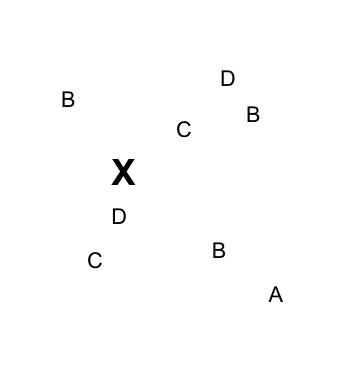
\includegraphics[width=\textwidth]{CM-ExampleLocation.png}
        \caption{\small A candidate location X has named objects A-D with the spatial layout depicted above.} 
        \label{fig:CM-LO-Example}
    \end{subfigure}
    \hfill
    \begin{subfigure}[t]{.25\textwidth}
        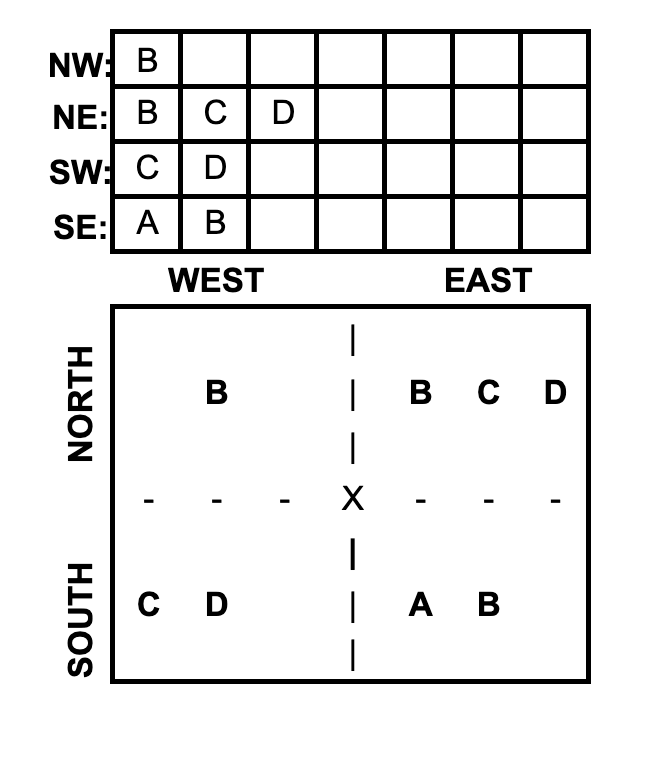
\includegraphics[width=\textwidth]{CM-LO-Setup.png}
        \caption{\small The objects are binned into spatial quadrants based on their relative position to the location coordinates, X.} 
        \label{fig:CM-LO-Setup}
    \end{subfigure}
    \hfill
        \begin{subfigure}[t]{.25\textwidth}
        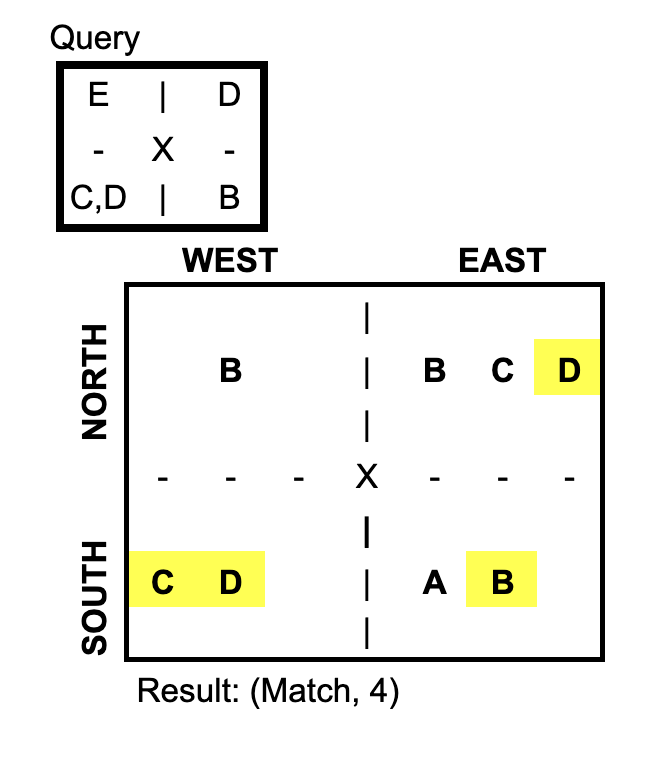
\includegraphics[width=\textwidth]{CM-LO-Query1.png}
        \caption{\small Rank the locations by the number of query terms that are found in the correct quadrant with respect to the location.}
        \label{fig:CM-LO-Query}
    \hfill
    \end{subfigure}
    \caption{\textbf{Object-Location Search Method. A Location-centric data structure (Figure \ref{fig:CM-LO-Setup}) is generated based on the cardinal relations between the objects and the location (Figure \ref{fig:CM-LO-Example}). Then a pictorial query is matched against the structure (Figure \ref{fig:CM-LO-Query}).}}\label{figure:ConceptMap-LO} 
\end{figure*}





\begin{figure*}[h]
    \centering
    \begin{subfigure}[t]{.25\textwidth}
        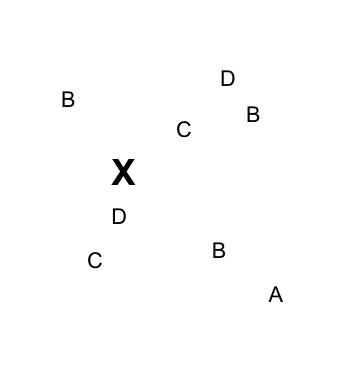
\includegraphics[width=\textwidth]{CM-ExampleLocation.png}
        \caption{\small A candidate location X has named objects A-D with the spatial layout depicted above.}
        \label{fig:CM-Example}
    \end{subfigure}
    \hfill
    \begin{subfigure}[t]{.25\textwidth}
        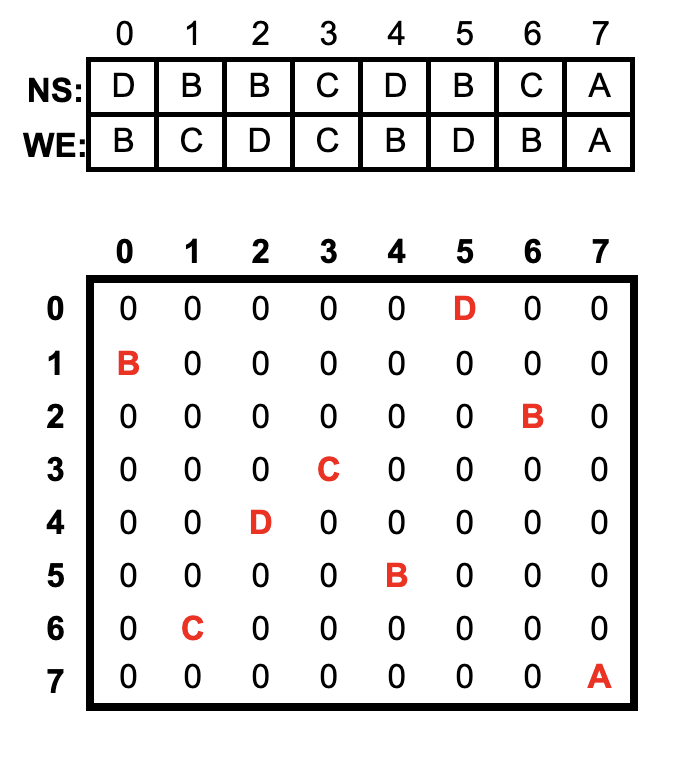
\includegraphics[width=\textwidth]{CM-OO-Setup.png}
        \caption{\small Objects associated with location X are ordered from North to South (NS) and West to East (WE) and mapped into a matrix with corresponding indices.}
        \label{fig:CM-OO-Setup}
    \end{subfigure}
    \hfill
        \begin{subfigure}[t]{.25\textwidth}
        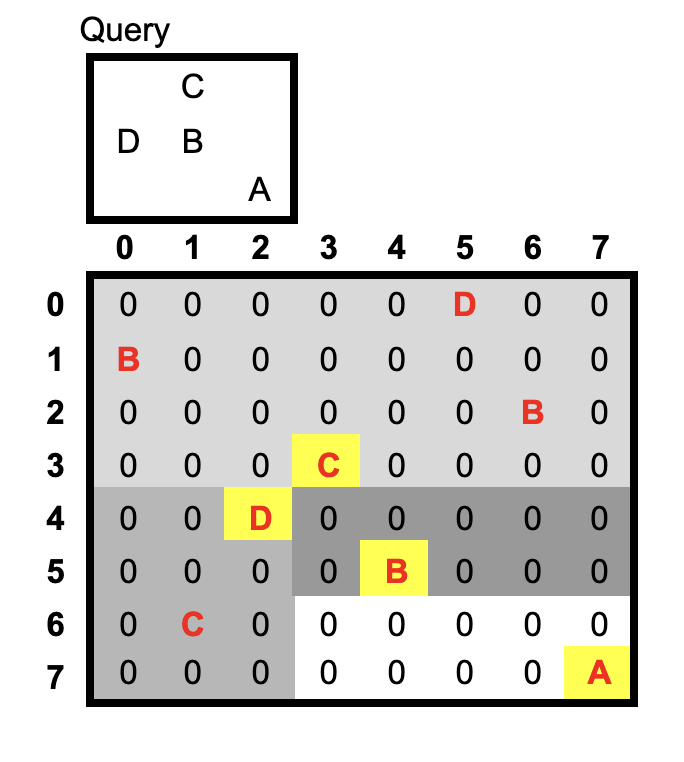
\includegraphics[width=\textwidth]{CM-OO-Query1.png}
        \caption{\small Recursive search. Each recursion is a darker shade, with an unpruned area in white. Objects highlighted in yellow are found to match the query configuration; candidate location X is a match for the query.}
        \label{fig:CM-OO-Query}
    \hfill
    \end{subfigure}
    \caption{\textbf{Object-Object Search Method. A Concept Map data structure (Figure \ref{fig:CM-OO-Setup}) is generated by ordering the objects associated with a candidate location (Figure \ref{fig:CM-Example}) from North to South and West to East. The search step (Figure \ref{fig:CM-OO-Query}) then recursively prunes the concept map until ANY matching configuration of objects is identified or the query constraints are not satisfied.
    }}\label{figure:ConceptMap} 
\end{figure*}